\begin{figure}[]
     \centering
     \begin{subfigure}[b]{0.47\textwidth}
         \centering
         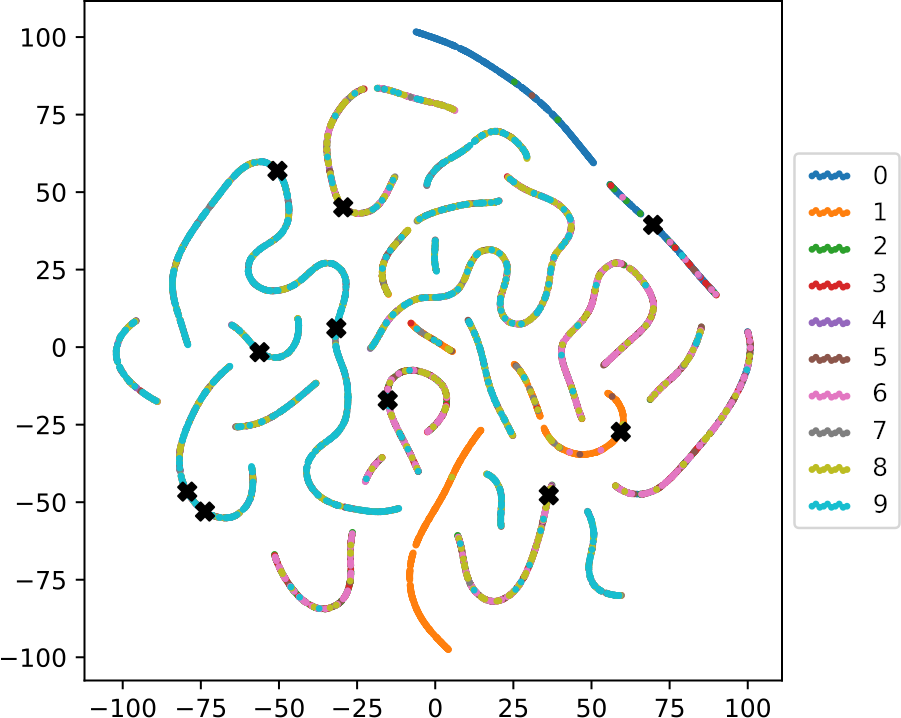
\includegraphics[width=\textwidth]{observational/img/vae/vae_TSNE_ls1.png}
         \caption{Latent size $=1$}
     \end{subfigure}
     \hfill
     \begin{subfigure}[b]{0.47\textwidth}
         \centering
         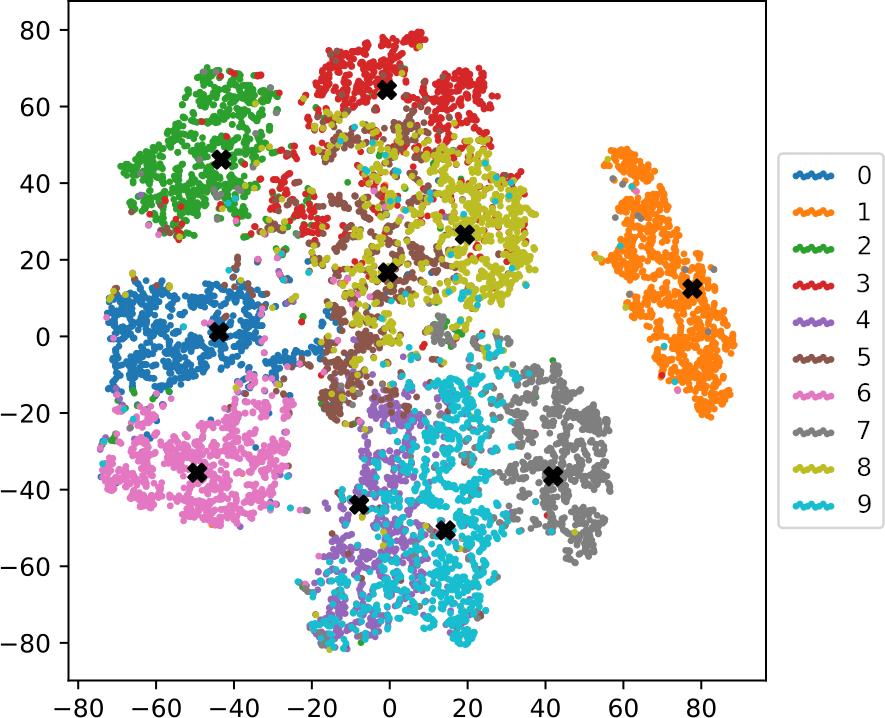
\includegraphics[width=\textwidth]{observational/img/vae/vae_TSNE_ls5.png}
         \caption{Latent size $=5$}
     \end{subfigure} 
     \par\bigskip
     \begin{subfigure}[b]{0.47\textwidth}
         \centering
         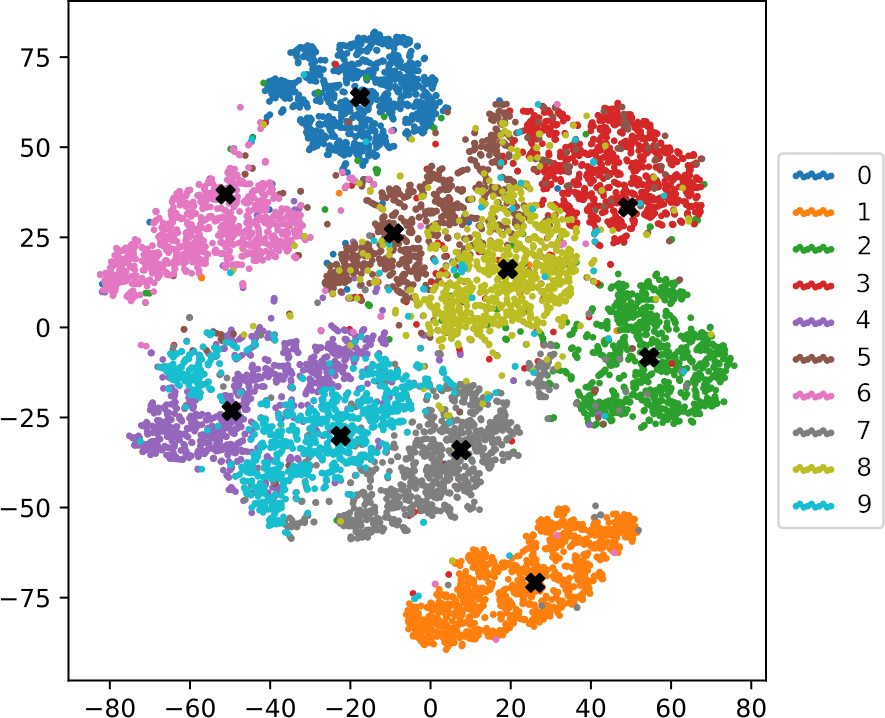
\includegraphics[width=\textwidth]{observational/img/vae/vae_TSNE_ls9.png}
         \caption{Latent size $=9$}
     \end{subfigure}
     \hfill
     \begin{subfigure}[b]{0.47\textwidth}
         \centering
         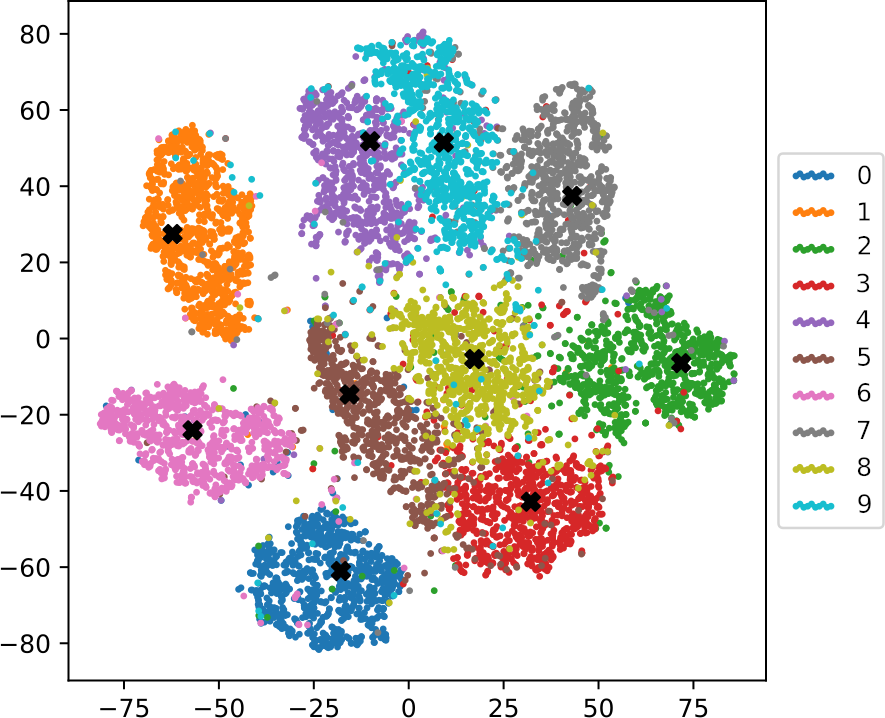
\includegraphics[width=\textwidth]{observational/img/vae/vae_TSNE_default.png}
         \caption{Latent size $=10$}
     \end{subfigure} 
     \par\bigskip
     \begin{subfigure}[b]{0.47\textwidth}
         \centering
         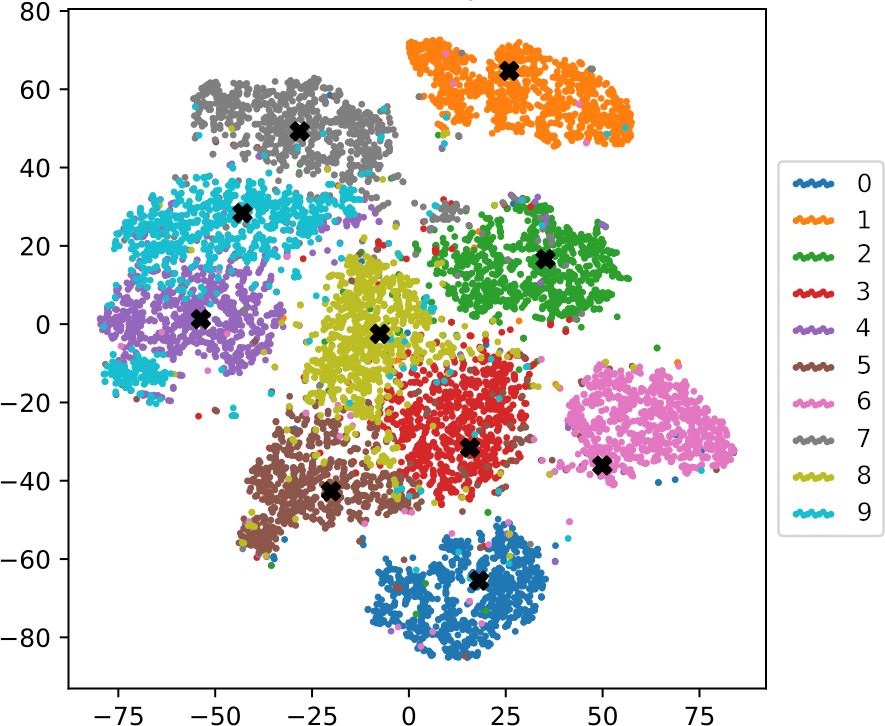
\includegraphics[width=\textwidth]{observational/img/vae/vae_TSNE_ls20.png}
         \caption{Latent size $=20$}
     \end{subfigure}
     \hfill
     \begin{subfigure}[b]{0.47\textwidth}
         \centering
         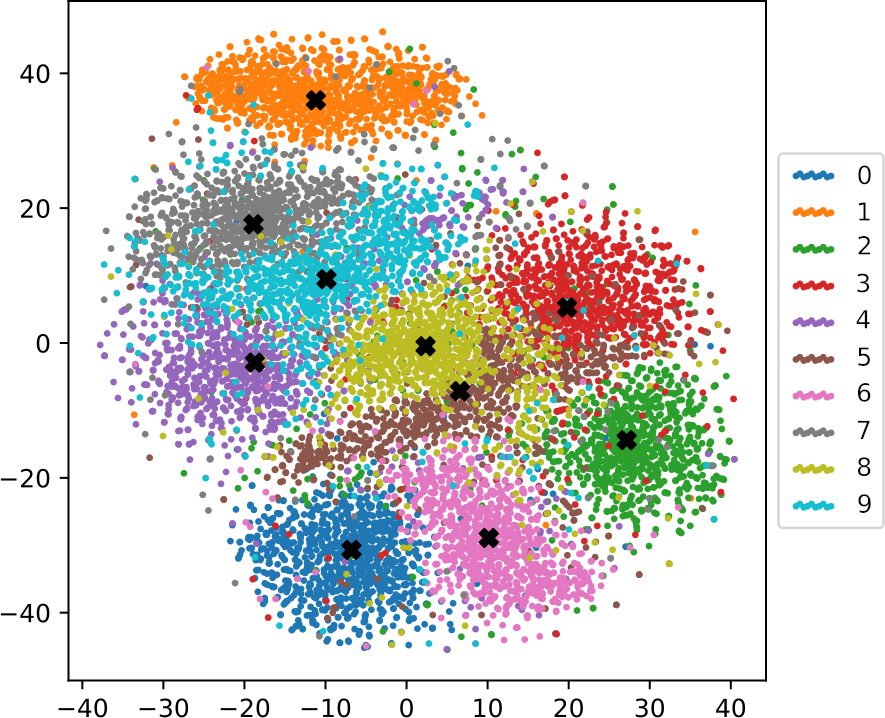
\includegraphics[width=\textwidth]{observational/img/vae/vae_TSNE_ls50.png}
         \caption{Latent size $=50$}
     \end{subfigure} 
     \caption[Latent size influence on VAE representation separability]{Latent size influence on Variational Autoencoder representation separability.}
    \label{fig:vae-tsne-latent}
\end{figure}
